\documentclass[]{report}
\usepackage{listings}
\usepackage[ngerman]{babel}
\usepackage[utf8]{inputenc}
\usepackage[pdftex]{graphicx}     
\usepackage{booktabs}
\usepackage{color}
\usepackage{tabulary}
\usepackage{url}

 \lstset{language=Java,
          showstringspaces=false,
          frame=single,
          numbers=left,
          basicstyle=\ttfamily\scriptsize,
          numberstyle=\tiny,
        }
% Title Page
\title{MISS \\ MAC-based Identification and Signaling Service}
\author{Universität Ulm \\ Institut für Datenbanken und Informationssysteme \\ \\ Fabian Schwab (fabian.schwab@uni-ulm.de)}
\begin{document}
\maketitle

%\begin{abstract}
%\end{abstract}
\chapter{Einleitung}
Um sich den Alltag zu erleichtern, werden immer mehr kleine Aufgaben auf mobile Endgeräte (z.B. Smartphone oder Tablet ausgelagert, und werden so zu unseren ständigen Begleitern. Der auf einem Smartphone genutzte Kalender enthält beispielsweise alle Termine und wichtige Aufgaben, welche an bestimmten Tagen zu gewissen Zeiten zu erledigen sind. Einfache Funktionen innerhalb dieser Kalenderanwendungen erlauben es, individuelle Benachrichtigungen für jeden Termin einzustellen, welche den Nutzer durch Audio-, Visuelle- oder Audiovisuelle-Benachrichtigungen an das bestimmtes Ereignis erinnern sollen. Doch solche zeitabhängigen Erinnerungen sind nicht immer praktisch für den Nutzer. In manchen Situationen lässt sich nicht genau festlegen, wann eine Aufgabe zu erledigen ist. Soll die Aufgabe zum Beispiel nach der Arbeit erledigt werden, kann man dies natürlich als zeitabhängiges Event einstellen. Verlässt man aber die Arbeit nicht zur gewohnten oder geplanten Zeit, kann diese Erinnerung zu spät erscheinen. Wird die Erinnerung zu früh ausgelöst kann es sein, dass der Nutzer sie vergisst. \\
Durch dieses Problem bedingt entstanden viele Anwendungen, welche auch ortsabhängige Erinnerungen durchführen können. So lassen sich beim Verlassen oder Ankommen an voreingestellten Orten Erinnerungen auslösen. Zum Beispiel wäre es so möglich einzustellen, dass beim Verlassen der Arbeit, eine entsprechende Erinnerung ausgelöst wird. \\
Mit diesen ortsgebundenen Erinnerungen lassen sich schon eine Vielzahl an möglichen Szenarien abdecken. Doch es gibt noch einen großen Teil, an Aufgaben, die weder Zeit noch Ortsgebunden bestimmt werden können. Dies trifft vor allem auf Szenarien im Zusammenhang mit anderen Personen zu. Es lässt sich oft schwer vorausahnen wann und wo man eine Person antrifft und damit entfallen orts- und zeitgesteuerte Erinnerungen. Einfache Notizen erscheinen hier noch das beste Mittel der Wahl zu sein. Doch an diese muss sich der Nutzer selbst erinnern. Dabei spielt der zeitliche Abstand der Notiz zum erneuten Treffen einer Person eine große Rolle. Je größer dieser Abstand ist, desto größer ist die Wahrscheinlichkeit, dass der Nutzer sich nicht mehr daran erinnert. \\
Bei diesen Szenarien wäre eine personenbezogene Erinnerung von Vorteil. Ein möglicher Ansatz, dies zu realisieren, wird in dieser Arbeit vorgestellt und diskutiert. \\ 
Um eine Person maschinell zu erkennen und zu bestimmen um wem es sich handelt, benötigt man einen einfachen Identifikator. Idealerweise ist dieser bereits digital und muss nicht aus analogen Werten, wie einer Geschichtserkennung oder ähnlichem gewonnen werden. Wie zu Beginn erwähnt, sind Smartphones und Tablets ständig griffbereit und heutzutage ein allgegenwärtiger Begleiter.\\
Da diese Geräte meist ohne Unterbrechung mit dem Internet verbunden sind, liegt die Lösung nahe, den Aufenthaltsort aller Nutzer auf einem zentralen Server zu speichern. Doch diese Lösung würde einige Probleme mit sich bringen. Unter anderem wäre das ständige Ermitteln und übermitteln des eigenen Standorts an diese zentrale Komponente unerlässlich. Das wiederum bedeutet einen hohen Energiebedarf und eine hohe Erneuerungsrate bei schnellen Ortswechseln. Auch müssten alle Nutzer die selbe Anwendung installiert haben um einen funktionsfähigen Dienst zu ermöglichen. \\
Selbst wenn diese Hürden überwindet werden würden, besteht noch immer die Gefahr, dass diese Positionsdaten missbraucht werden könnten. Die Sicherheitsmaßnahmen müssten enorm hoch sein um ein solches System gegenüber Missbrauch zu schützen. Ebenfalls müssten alle Nutzer ihr Vertrauen in dieses System setzten. Würden Nutzer ihre Internetverbindung für solch eine Anwendung absichtlich sperren oder hätten keinen Empfang, so könnte auch dieser Ansatz nicht mehr funktionieren.\\ \\
Ein dezentraler Ansatz, welcher keine ständige Internetverbindung benötigt und von jedem Nutzer kontrolliert werden könnte wäre somit die bessere Lösung. Um zu wissen ob sich eine Person in der Nähe befindet ist nicht die genaue Position interessant, sonder lediglich die Distanz zu dieser Person beziehungsweise zu ihrem mobilen Endgerät. Genau auf dieser Grundlage entstand das Projekt \textit{MAC-based Identification and Signaling Service} (kurz MISS).\\
Jedes WLAN-fähige Gerät muss sich beim Senden oder Empfangen von Daten, aber auch in regelmäßigen Abständen mit anderen WLAN-Geräten in der Nähe abstimmen, ob bzw. wann die Luftschnittstelle frei zur Übertragung von Daten ist. Genau diese Kommunikation kann genutzt werden um Geräte in der Nähe zu erkennen und identifizieren.\\ 
Die einzige Information die dazu benötigt wird, ist die MAC-Adresse des zu suchenden Gerätes. Dabei hat der Besitzer des Gerätes die volle Kontrolle, wem er diese Adresse mitteilt. \\
Der \textit{MAC-based Identification and Signaling Service} ist ein für Android geschriebener Hintergrunddienst, der es ermöglicht WLAN Geräte zu erkennen. Der Service unterscheidet dabei zwischen mobilen Geräten (hier als \textit{Clients} bezeichnet), und Stationen (sogenannten \textit{Stations}). Hierbei sind die \textit{Clients} Geräte die sich mit einem WLAN verbinden und \textit{Stations} die solch ein Netzwerk aufspannen. Je nach Typ, also \textit{Client} oder \textit{Station}, werden verschiedene Informationen, wie beispielsweise Signalstärke oder \textit{ESSID} gesammelt und übermittelt. Diese Informationen werden in Kapitel \ref{lab:airodump-ng} genauer erläutert und beschrieben.\\
Sobald sich eines der gesuchten Geräte in der Nähe befindet und erfolgreich identifiziert wird, kann eine Benachrichtigung über die Anwesenheit einer damit verknüpften Person, ausgelöst werden.
\chapter{Grundlagen}
Um die Funktionsweise des entwickelten Services genauer verstehen zu können, werden zunächst einige Grundlagen erklärt. In diesem Kapitel werden die vom Service genutzten Technologien  beschrieben. Da dies keine vollständige Beschreibung darstellt, sollten die verwendeten Technologien in ihren Grundzügen bereits bekannt sein. 
\section{Kabellose Kommunikation}
Die Anzahl der Geräte die mithilfe von WLAN kommunizieren nehmen ständig zu. Bei einem Großteil dieser Geräte wird der \textit{WNIC}\footnote{Wireless Network Interface Controller}, manchmal trotz limitierter Ressourcen, nicht abgeschaltet. Trotz verschlüsselter Verbindungen, werden durch den \textit{IEEE 802.11} Standard \cite{IEEE} definiert, einige Daten in Klartext übertragen. Diese Daten werden von MISS genutzt um Geräte in der Nähe zu erkennen und bereits bekannte Geräte zu identifizieren. \\
Durch den \textit{IEEE 802.11} Standard werden auf der Sicherungsschicht des \textit{OSI-Modells} \cite{OSI}  Datagramme, sogenannte \textit{Frames} definiert welche in spezielle Teile unterteilt sind. Jeder \textit{Frame} enthält ein \textit{MAC-Header} Feld, in dem die Absender MAC-Adresse im Klartext dargestellt ist. Durch abhören der umliegenden Kommunikation kann so nach einer bestimmten MAC-Adresse gesucht werden. \\
Aber nicht nur Geräte die gerade aktuell Daten austauschen, können so erkannt werden, sonder, auch Geräte die gerade inaktiv sind. Jedes WLAN-fähige Gerät sendet, abhängig von der Implementierung des \textit{WNIC} Treibers, periodisch Pakete aus. Diese Pakete gehören zu der Gruppe der \textit{Managementframes} welche im nachfolgenden Listing aufgeführt sind. \\
\begin{itemize}
	\item Beacon Frame
	\item Probe Request Frame
	\item Probe-Response Frame
	\item Authentication Frame
	\item Association Request frame
	\item Authentication Response
	\item Disassociation frame
	\item Deauthentication frame
	\item Reassociation Request frame
	\item Reassociation Response frame
\end{itemize}
Bei den \textit{probe request frames} handelt es sich um Pakete, die von \textit{Clients} gesendet werden, um Informationen über naheliegende Netzwerke zu sammeln. Durch die Angabe einer \textit{SSID}\footnote{Service Set Identifier} kann im Kommunikationsbereich des Gerätes nach bestimmten Netzwerken gesucht werden. Durch die Angabe der \textit{broadcast SSID} kann nach allen Netzwerken gesucht werden, die dieses Paket empfangen und darauf antworten. Diese Pakete werden versendet, egal ob das Gerät bereits mit einem Netzwerk verbunden ist oder nicht.\\
\textit{Stations} senden sogenannte \textit{beacon frames} aus. Damit geben sie periodisch ihre Präsenz, \textit{SSID} und andere Parameter bekannt. \\
Im Standard Betriebsmodus eines \textit{WNIC} ist es nicht vorgesehen, dass Pakete, die an andere MAC-Adressen gerichtet sind an höhere Schichten des \textit{OSI-Modells} weitergeleitet werden. Diese Pakete werden bereits auf der zweiten Schicht, dem \textit{Data Link Layer}, im \textit{WNIC} verworfen. Damit aber auch diese Pakete weitergeleitet werden, ist es notwendig den Betriebsmodus des \textit{WNIC} in den sogenannten \textit{Monitor Mode} zu versetzten. Dieser Modus kann über den Treiber des \textit{WNIC} eingestellt werden und muss dort auch implementiert sein. 
\subsection{Airodump-ng}\label{lab:airodump-ng}
\textit{Airodump-ng} \cite{Airodump-ng} ist ein Kommandozeilenprogramm welches für das Erfassen von \textit{IEEE 802.11 frames} genutzt wird und ist Bestandteil der \textit{Aircrack-ng suite} \cite{Aircrack-ng}. Mit diesem Programm lassen sich Log-Dateien erstellen, welche Informationen über alle erfassten \textit{Stations} und \textit{Clients} enthalten. Eine Auszug einer solchen Log-Datei ist in Abbildung \ref{fig:log_file} zu sehen. Die Tabellen \ref{tab:1} und \ref{tab:2} beschreiben die erfassbaren Daten für \textit{Stations} und \textit{Clients} \cite{Airodump-ng}.\\ \\
\begin{figure}
    \centering
    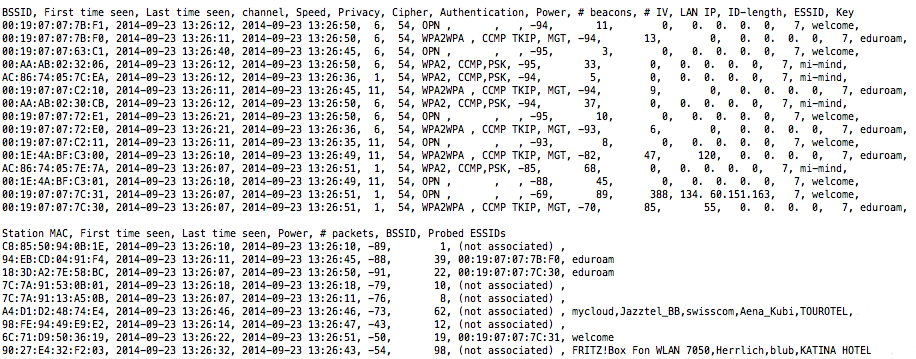
\includegraphics[width=5.0in]{bilder/log.png}
    \caption{Mit airodump-ng erstellte Log-Datei}
    \label{fig:log_file}
\end{figure}
\begin{center}
\begin{table}
\caption{Stationdaten}\label{tab:1}
  \begin{tabulary}{\textwidth}{l | L}
\toprule
Erfassbare \textit{Station} Daten & Beschreibung \\
\midrule
BSSID & MAC-Adresse der \textit{Station} \\
First time seen & Datum und Uhrzeit der ersten Kontakts \\
Last time seen & Datum und Uhrzeit des letzten Kontakts \\
Channel &  Kanal auf der die \textit{Station} sendet \\
Speed & Übertragungsgeschwindigkeit in MBit/s\\
Privacy & Privatsphäreneinstellungen \\
Cipher & Art der Verschlüsselung \\
Authentication & Genutztes Authentifizierungsprotokoll \\
Power & Signalstärke \\ 
Anzahl beacons & Anzahl der Empfangenen \textit{beacon frames}\\
Anzahl IV & Anzahl der Erkannten Initialisierungsvektoren \\
LAN IP &  IP Adresse \\
ID-length & Zeichenanzahl ESSID \\
ESSID & Netzwerkname \\
Key & Netzwerkschlüssel falls bekannt\\
\bottomrule
\end{tabulary}
\end{table}
\end{center} 
\begin{center}
\begin{table}
\caption{Clientdaten}\label{tab:2}
  \begin{tabulary}{\textwidth}{l | L}
\toprule
Erfassbare \textit{Client} Daten & Beschreibung \\
\midrule
Station MAC & MAC-Adresse\\
First time seen & Datum und Uhrzeit der ersten Kontakts \\
Last time seen & Datum und Uhrzeit der letzten Kontakts \\
Power & Signalstärke \\
Anzahl packets & Anzahl der Empfangenen \textit{frames} \\
BSSID & BSSID mit dem der \textit{Client} verbunden ist \\
Probed ESSIDs & ESSID die der \textit{Client} sucht \\
\bottomrule
\end{tabulary}
\end{table}
\end{center}
\section{Android}
Bevor der eigentliche Hintergrunddienst installiert werden kann, müssen einige Vorbereitungen getroffen werden. Da Google in seinem offenen Betriebssystem Android keine Möglichkeit bietet den \textit{Monitor Mode} explizit zu aktivieren, implementieren die Hersteller in ihren Gerätetreibern diesen meist auch nicht.\\
Zum Zeitpunkt dieses Projekts gibt es kein Android Gerät, welches einen \textit{WNIC} besitzt, für den es einen vom Hersteller implementierten \textit{Monitor Mode} gibt. \\
Für bestimmte Chipsätze des Herstellers Broadcom \cite{Broadcom} gibt es eine kleine Gruppe von Programmierer, die für die Chipsätze \textit{BCM4330} \cite{BCM4330} und \textit{BCM4329} \cite{BCM4329} eine neue Firmware geschrieben haben um eben diesen Modus zu aktivieren. Momentan werden folgende Geräte mit diesem Chipsatz ausgeliefert \cite{bcmonBlog}:
\begin{itemize}
\item Samsung Galaxy GS1 mit Cyanogen 7
\item Samsung Galaxy GS2 mit Cyanogen 9 oder Cyanogen 10
\item HTC Nexus One mit Cyanogen 7
\item Asus Nexus 7 mit Cyanogen 7
\end{itemize}
\subsection{Cyanogen}
Alle zuvor aufgelisteten Geräte nutzen Cyanogen \cite{Cyanogen}. Cyanogen ist eine erweiterte \textit{open source} Firmware Distribution für Smartphones und Tablets, welche auf dem Android Betriebssystem basiert. Cyanogen bietet Eigenschaften und Erweiterungen die es in der offiziellen Android oder in der von Herstellern ausgelieferten Firmware nicht gibt. \\
Um Cyanogen auf einem unterstützten Gerät zu installieren, muss dies zuvor \textit{gerootet} werden. Diese bedeutet, das man alle Rechte erlangt was normalerweise, auch aus Sicherheitsgründen, von Google nicht vorgesehen ist. 
\subsection{bcmon.apk}
Nachdem das Gerät \textit{gerootet} und Cyanogen installiert wurde, kann man ein zusätzliches Programm installiert werden, mit dessen Hilfe der \textit{Monitor Mode} aktiviert werden kann. Das Programm \textit{bcmon} \cite{bcmon.apk} enthält dabei eine neuen Treiber für den \textit{WNIC} in dem der \textit{Monitor Mode} und weitere Modi implementiert sind. Anschließend ist das Gerät für die Verwendung des MISS Hintergrunddienstes vorbereitet. 
\chapter{Architektur und Implementierung}
In diesem Kapitel wird zunächst die grundlegende Architektur des verwendeten Dienstes erläutert und anschließend auf die Implementierung des Service eingegangen. Für diese Kapitel werden Grundlagen der Programmierung in Java und Android vorausgesetzt. Sind diese nicht vorhanden, wird an dieser Stelle auf die Android-Entwicklerseite \cite{AndroidDeveoper} verwiesen. 
\section{Architektur}
Dieses Kapitel erklärt die Funktionsweise des Service, so wie seine Implementierung. Der Quellcode dieses Projekts ist gut Dokumentiert und für das Verständnis dieses Kapitels hilfreich aber nicht Voraussetzung. 
\subsection{Android Bound Service}
Ein Service ist eine im Hintergrund laufende Komponente welche keine direkte Interaktion mit einem Nutzer besitzt. Da ein Service keine Benutzeroberfläche benötigt, ist dieser auch nicht an den normalen Lebenszyklus einer \textit{Activity} gebunden. Im Allgemeinen werden Services genutzt um wiederkehrende und potentiell lange andauernde Aufgaben zu erledigen, wie beispielsweise das Herunterladen von Inhalten aus dem Internet oder das Aktualisieren von Daten. Ebenfalls werden Services mit einer höheren Priorität ausgeführt, als Anwendungen die sich im Hintergrund befinden. Somit ist es unwahrscheinlicher, dass sie vom Betriebssystem abgeschaltet werden. \\
Zusätzlich können Services unter Android so konfiguriert werden, dass sie neu gestartet werden sollte das Betriebssystem den Service beenden. \\
Da der in diesem Projekt genutzte Service nicht immer aktiv sein soll, wird hier auf eine besondere Art eines Services zurückgegriffen. Bei dieser Art von Hintergrunddienst handelt es sich um einen \textit{Bound Service} \cite{BoundService}, welcher von der selben Klasse wie ein normaler \textit{Service} erbt. \\
Man kann einen \textit{Bound Service} als Server einer Client-Server-Kommunikation betrachten. Dies ermöglicht es anderen Komponenten sich an einen Service zu binden und so Anfragen zu senden und Antworten zu erhalten. Ebenso kann durch dies eine \textit{Interprocess Communication (IPC)} realisiert werden, was bei normalen Services nur mit erhöhtem Aufwand oder der \textit{Android Interface Definition Language (AIDL)} möglich wäre. \\
Um zwischen einem herkömmlichen und einem \textit{Bound Service} zu unterscheiden, müssen lediglich verschiedene Methoden implementiert werden. Die Lebenszyklen eines \textit{Service} und eines \textit{Bound Service} sind in Abbildung \ref{fig:lifetime} abgebildet. \\
Hierbei wird ersichtlich, dass diese Art von Service nicht immer im Hintergrund aktiv ist. Nur wenn ein Client an den Service gebunden ist, wird dieser aktiv. Im Gegensatz zu einem herkömmlichen Service, bei dem ein Aufruf von \texttt{stopService()} genügt um diesen zu beenden, wird ein \textit{Bound Service} erst beendet, wenn sich alle Clients abgemeldet haben.
\begin{figure}
    \centering 
    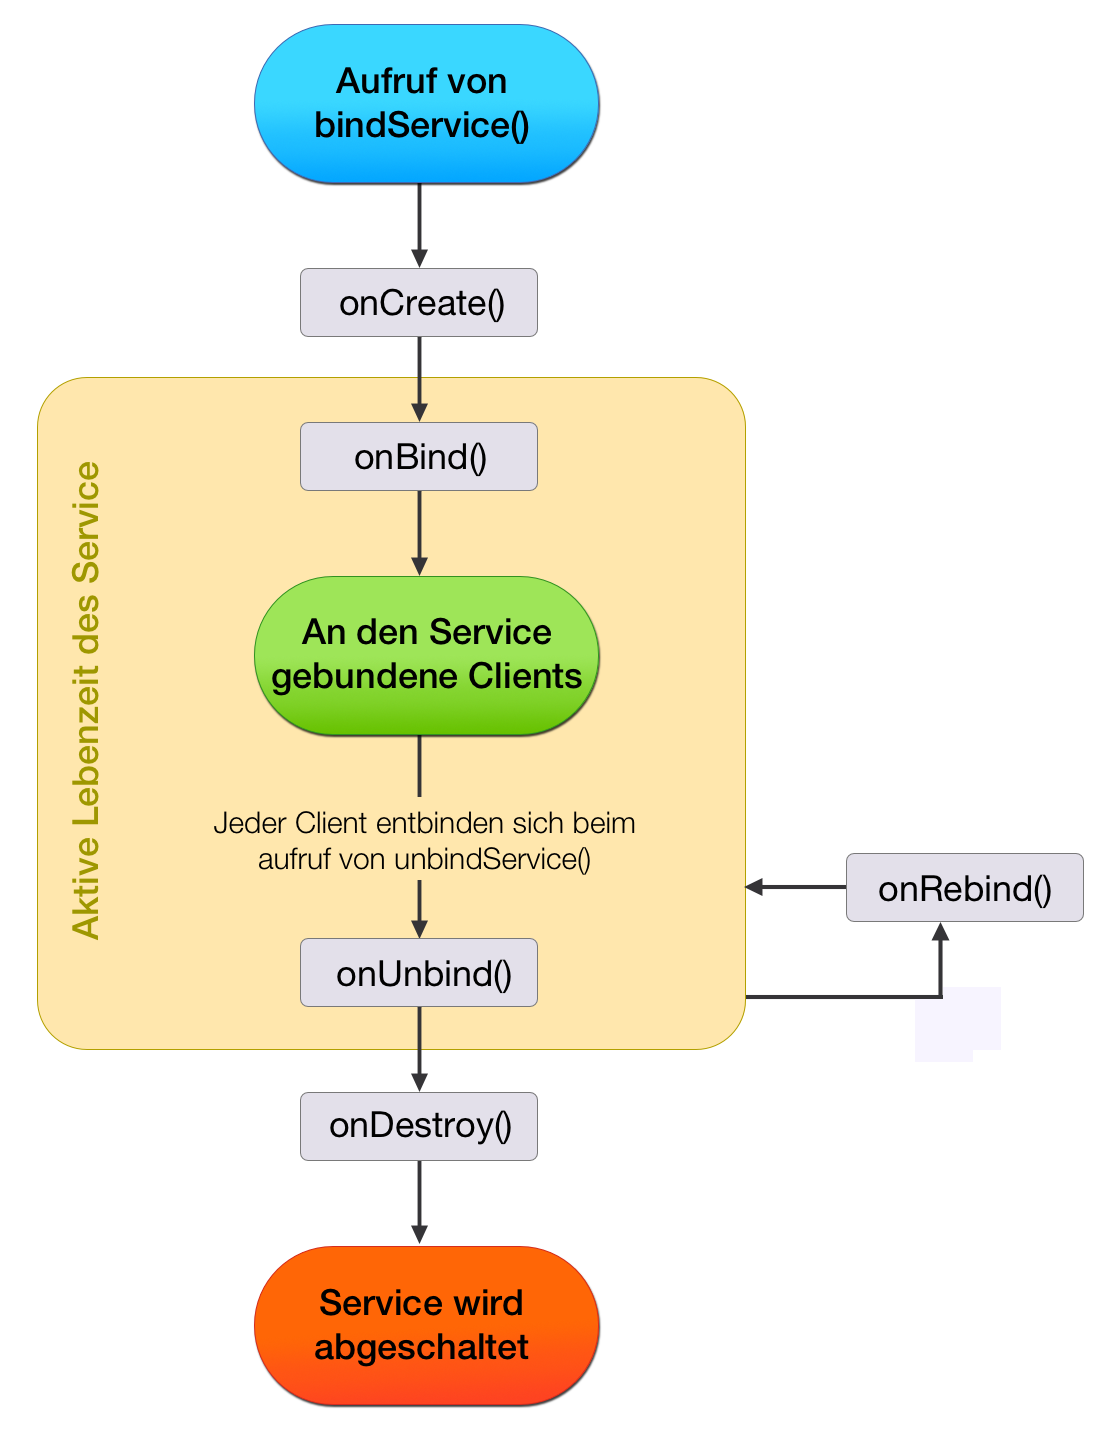
\includegraphics[width=3.0in]{bilder/boundservice.png}
    \caption{Lebenszyklus eines \textit{Service} (links) und \textit{Bound Service} (rechts) \cite{android}}
    \label{fig:lifetime}
\end{figure}
\subsection{Service Logik}
Die Kommunikation der Komponenten, wie sie im Service implementiert wurden ist in Abbildung \ref{fig:uml} ersichtlich. Bindet sich eine Anwendung an den Service, wird dieser gestartet, sofern dieser nicht bereits aktiv ist. Der Service läuft als eigenständiger Prozess und verfügt über einen zusätzlichen Thread, welcher die eigentliche Arbeit übernimmt. Dies ermöglicht ein sofortiges Abarbeiten ankommender Anfragen im Hauptprozess von bereits gebundenen Anwendungen oder solchen, die sich gerade an den Service binden möchten. \\
Aus Effizienzgründen wird der Arbeiter-Thread nur dann gestartet wenn Geräte in der Umgebung gesucht werden. Zu suchenden Geräte werden dann über Nachrichten an den Service übermittelt, der daraufhin den Thread nach Bedarf startet oder stoppt. \\
Die Aufgabe des Threads ist es, alle Geräte in der Nähe des eigenen Geräts zu erfassen. Dabei werden alle zu erfassenden Daten, wie in Abschnitt \ref{lab:airodump-ng} gezeigt, ausgelesen und protokolliert. Anschließend werden die gefunden Geräte mit denen verglichen, für die eine Erinnerung definiert und erstellt wurde. Befindet sich solch ein Gerät unter den entdecktet Geräten, so benachrichtigt der Arbeiter-Thread den eigentlichen Service. Dieser wiederum sendet eine Nachricht an die entsprechende Anwendung und informiert diese über den Fund des angefragten Gerätes. \\ 
Je nach Implementierung der Zielanwendung entscheidet diese über das weitere Vorgehen. In der Regel wird davon ausgegangen, dass die Anwendung das gesuchte Gerät nicht mehr benötigt, da eine Aktion ausgelöst wurde. Damit der Service das Gerät nicht weiterhin sucht, muss dies an den Service übermittelt werden.  
Durch eine Nachricht welche die Anwendung an den Service sendet, wird das zuvor gesuchte Gerät entfernt.\\
Der Service überprüft dem Empfangen einer Nachricht, ob der Arbeiter-Thread gestartet werden muss oder nicht. Sind keine Geräte mehr vorhanden wird der Thread automatisch beendet. Antwortet eine Anwendung auf den Fund eines Gerätes nicht, wird davon ausgegangen, dass die Anwendung unerwartet beendet wurde. Der Service entfernt die Anwendung und alle mit dieser in Verbindung stehenden Geräte.\\
Befinden sich danach keine gesuchten Geräte mehr im Dienst, beendet dieser den Arbeiter-Thread um Ressourcen an das Betriebssystem freizugeben. Haben sich alle Anwendungen ordnungsgemäß vom Service abgemeldet oder wurden durch eine ausbleibende Antwort entfernt, beendet sich der Service selbst da er nun nicht mehr benötigt wird.
\newpage
\begin{figure}[h!]
    \centering 
    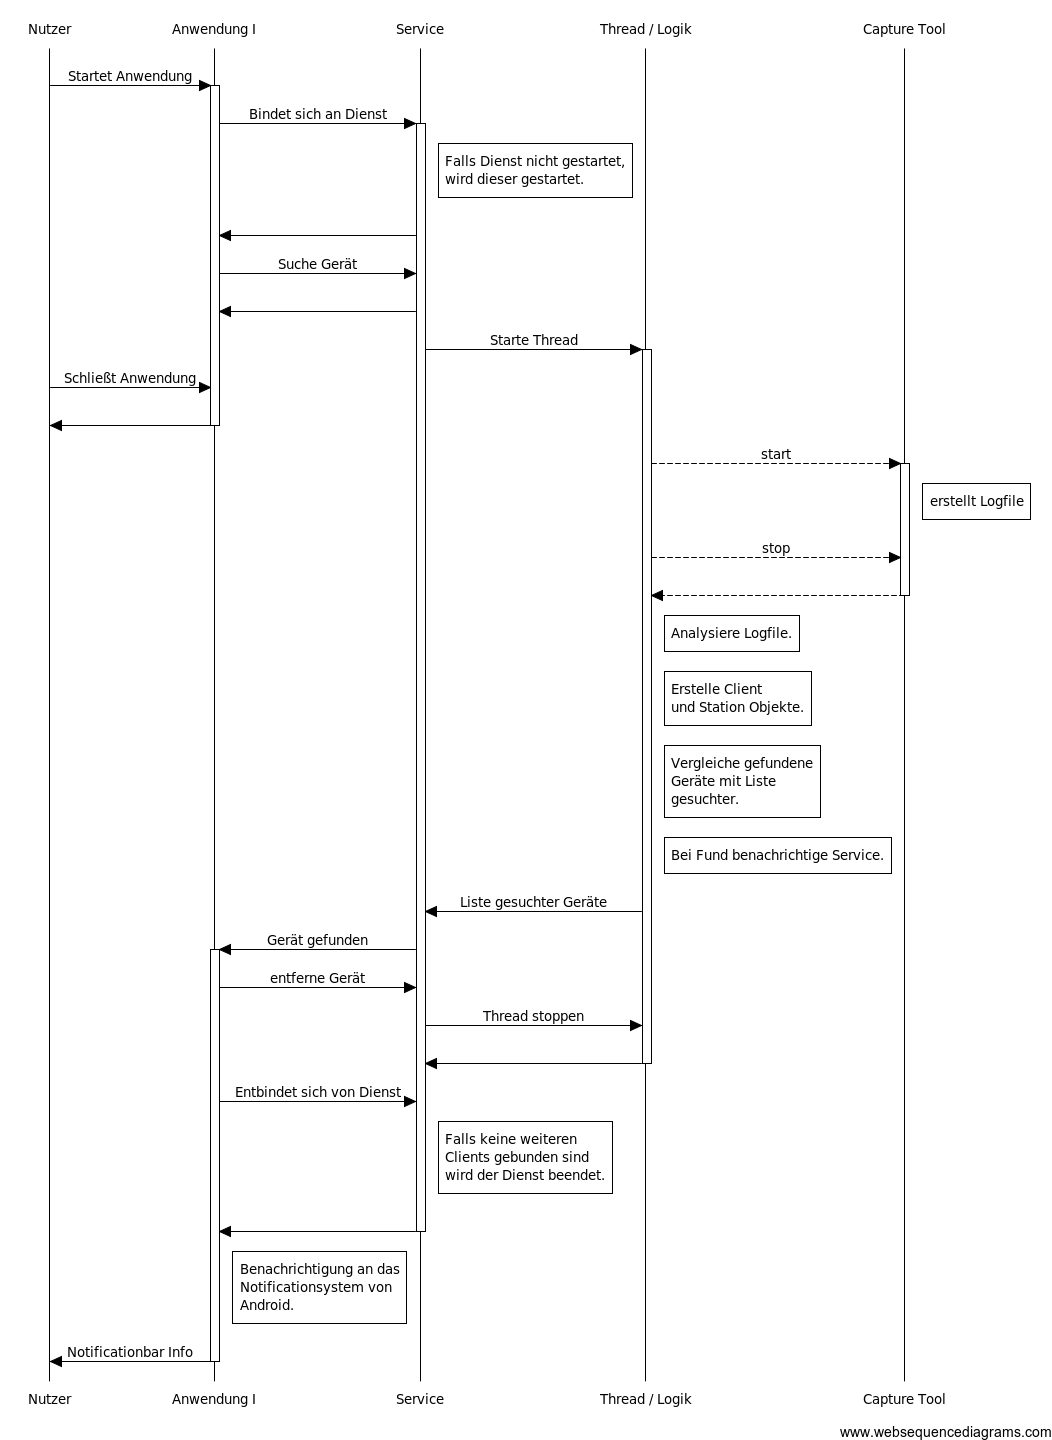
\includegraphics[width=5.0in]{bilder/uml.png}
    \caption{Anwendungsfall und Lebenszyklus des MISS als UML-Sequenzdiagramm.}
    \label{fig:uml}
\end{figure}
\section{Implementierung}
Für die Implementierung des erläuterten Ablaufs wurde das Eclipse ADT \cite{ADT} verwendet. Als Zielgerät wurde das Samsung Galaxy GS1 \cite{S1} mit Cyanogen 7 gewählt. Hierbei war zu beachten, das bei der Programmierung nur Methoden bis API Level 10 genutzt werden konnten. Dies liegt an der niedrigen Android Version 2.3.3 welche dem Cyanogen 7 Mod zu Grunde liegt. \\
Da im späteren Betrieb des Service Skripte benötigt werden, wurden diese zur besseren Kapselung und Entwicklung als \texttt{.sh} Datei im \texttt{assets} Ordner gespeichert. Dies hat den entscheidenden Vorteil, dass diese von der Anwendung automatisch generiert werden können und nicht nach der Installation von Nutzer im entsprechenden Programmverzeichnis abgelegt werden müssen.\\ Ist die Luftschnittstelle auf einem anderen Gerät nicht unter der Standard Bezeichnung \texttt{wlan0} zu finden, so kann dies in den Skripts des Projekts einfach geändert werden. \\ 
Folgende Skripts werden bei der Installation erstellt:
\begin{itemize}
\item \texttt{removeCaptureFiles.sh} - entfernt Log-Dateien.
\item \texttt{startCapture.sh} - startet das Aufzeichnen der umliegenden Kommunikation.
\item \texttt{stopCapture.sh} - stoppt das Aufzeichnen.
\end{itemize}
Diese Skripts werden ausschließlich vom Arbeiter-Thread genutzt. Um eine unnötige Speicherbelegung zu vermeiden dient das \texttt{removeCaptureFiles.sh} Skript, welches die anfallenden Log-Datei entfernt. \\ Das Starten und Stoppen von \textit{airodump-ng} wird durch die beiden anderen Skripte veranlasst, wobei \texttt{startCapture.sh} wie in Listing \ref{lst:sh} einige Parameter beim Aufruf enthält. So wird hier das Ausgabeformat festgelegt und der \textit{WNIC} Name angegeben. Zusätzlich werden die fehlenden Umgebungsvariablen ergänzt, um gewisse Bibliotheken für \textit{airodump-ng} bereitzuhalten,
\begin{lstlisting}[caption={Airodump-ng Parameter}\label{lst:sh},captionpos=t] 
export PATH = $PATH:/data/data/com.bcmon.bcmon/files/tools
export LD_LIBRARY_PATH = 
  $LD_LIBRARY_PATH:/data/data/com.bcmon.bcmon/files/libs
export LD_PRELOAD = /data/data/com.bcmon.bcmon/files/libs/libfake_driver.so
airodump-ng -w /datadata/de.uulm.miss/files/capture 
  --output-format csv -w capture wlan0 2>&1
 \end{lstlisting}
In der Tabelle \ref{javaClass} werden alle Klassen inklusive einer dazugehörigen Beschreibung von MISS aufgeführt.
Auf eine ausführliche Beschreibung der einzelnen Funktionen und Parameter wurde an dieser Stelle verzichtet, da diese aus dem Quellcode entnommen werden kann. Um diesen Service zu nutzen  können kann die beiliegende Anwendung \textit{PAR}, welche in Abschnitt \ref{lab:par} erläutert wird, genutzt werden. \\
Die Basisfunktionen die der Service als Schnittstelle anbietet werden im nächsten Kapitel \ref{lab:usage} erklärt. 
\begin{center}
	\begin{table}
		\caption{Übersicht von essentiellen Klassen}\label{javaClass}
		\begin{tabulary}{\textwidth}{l | L}
			\toprule
			Klassenname & Beschreibung \\
			\midrule
			MainActivity.java & Wird nur bei der Installation geöffnet und erzeugt alle benötigen Skripte und legt diese im entsprechenden Ordner ab.\\
			MISService.java & Nimmt Anwendungsanfragen entgegen, erzeugt und kontrolliert den Arbeiter-Thread. \\
			ScanLogic.java & Arbeiter-Thread der mithilfe der Skripte alle Geräte in der Umgebung findet und mit zu suchenden Geräten vergleicht. \\
			FileParser.java & Erstellt Client und Station Objekte aus Logfiles. \\
			Client.java & Objekt mit allen erfassbaren Daten. \\
			Station.java & Objekt mit allen erfassbaren Daten. \\ 
			ScanOrder.java & Enthält die Liste von gesuchten Stations und Clients. \\
			\bottomrule
		\end{tabulary}  
	\end{table}
\end{center}
\subsection{Nutzung des Service}\label{lab:usage}
Für die Nutzung des Service müssen folgende Punkte erfüllt sein:
\begin{itemize}
\item Ein unterstützter Chipsatz (\texttt{BCM4330} bzw. \texttt{BCM4329}) wurde verbaut.
\item Das Gerät ermöglicht \textit{root} Zugriff.
\item Eine kompatible Cyanogen Firmware ist aufgesetzt.
\item Die \textit{bcmon} Anwendung ist installiert.
\item Der Service MISS ist installiert und \textit{root} Rechte wurden bewilligt.
\item Der \textit{Monitor Mode} wurde über \textit{bcmon} aktiviert.
\end{itemize}
Für eine Nutzung von MISS innerhalb einer Anwendung müssen nicht viele Änderungen an dieser vorgenommen werden. Die Klasse welche mit dem Service letztendlich kommunizieren soll, muss das Interface \texttt{ServiceConnection} implementieren.\\
Hierbei müssen die beiden Methoden:
\begin{itemize}
\item \texttt{onServiceConnected(ComponentName name, IBinder service)}
\item \texttt{onServiceDisconnected(ComponentName name)}
\end{itemize}
implementiert werden. Erstere wird aufgerufen, wenn die Verbindung zum Service erfolgreich aufgebaut wurde, letztere, wenn die Verbindung zum Service unerwartet abbricht oder beendet wurde. \\
\subsubsection{An Service binden}
Listing \ref{lst:bind}  zeigt, wie eine Anwendung an den Service gebunden wird. Das \texttt{ServiceConnection} Objekt ist die \texttt{Aktivity} welche \texttt{ServiceConnetion} implementiert. Durch den Aufruf von \texttt{bindService()} wird die Anwendung an den Service gebunden und die Methode \texttt{onServiceConnected()} wird aufgerufen. 
\begin{lstlisting}[caption={Anwendung an Service binden.}\label{lst:bind},captionpos=t] 
ServiceConnection mConnection = this;
Intent mIntent = new Intent("de.uulm.miss.MISService");
bindService(mIntent, mConnection, Context.BIND_AUTO_CREATE);
\end{lstlisting}
An dieser Stelle wird ein Objekt vom Typ \texttt{Messenger} benötigt. Dieses Objekt ermöglicht eine Umsetzung für eine nachrichtenbasierte Kommunikation über Prozesse hinweg. Somit lassen sich Nachrichten an den Service übermitteln und von diesem entgegen nehmen. Das \texttt{Messenger} Objekt wird wie in Listing \ref{lst:msg} initialisiert wobei sich die Anwendung gleich am Service registriert. Dies wird mittels einer Nachricht an den Service realisiert. Der Service unterschiedet die verschiedenen Nachrichtentypen anhand der mitgesendeten Konstanten.
\begin{lstlisting}[caption={Registrieren der Anwendung am Service}\label{lst:msg},captionpos=t] 
...
private final Messenger mMessenger = 
  new Messenger(new IncomingMessageHandler(this));
...
@Override
public void onServiceConnected(ComponentName name, IBinder service) {
  mServiceMessenger = new Messenger(service);
  try {
    Message regMessage = Message.obtain(null, MSG_REGISTER_APPLICATION);
    regMessage.replyTo = mMessenger;
    mServiceMessenger.send(regMessage);
  } catch (RemoteException e) {
 	// In diesem Fall wurde der Service unerwartet beendet,
 	// bevor etwas mit ihm gemacht werden konnte.
  }
}
\end{lstlisting}
 Die Konstanten mit denen zwischen Anwendung und Service kommuniziert werden kann, werden nachfolgenden aufgeführt.
\begin{itemize}
\item \texttt{MSG\_REGISTER\_APPLICATION} - Anwendung an Service binden.
\item \texttt{MSG\_UNREGISTER\_APPLICATION} - Anwendung am Service abmelden.
\item \texttt{MSG\_ADD\_CLIENT} - Ein neu zu suchenden \textit{Client} am Service hinzufügen.
\item \texttt{MSG\_ADD\_STATION} - Eine neue zu suchende \textit{Station} am Service hinzufügen. 
\item \texttt{MSG\_REMOVE\_CLIENT} - Ein \textit{Client} aus dem Service entfernen.
\item \texttt{MSG\_REMOVE\_STATION} - Eine \textit{Station} aus dem Service entfernen.
\item \texttt{MSG\_FOUND\_DEVICE} - Ein entsprechendes Gerät wurde bei einem Suchlauf gefunden. 
 \end{itemize}
 Um auch eine Antwort verarbeiten zu können, muss wie in Listing \ref{lst:msg} in Zeile 2 \& 3 ein \texttt{Messenger} Objekte erstellt werden. Die Klasse \texttt{IncomingHandler} erbt von \texttt{Handler}. Dabei muss die Methode \texttt{handleMessage()} überschrieben werden, um die vom Entwickler gewünschten Aktionen durchführen zu können. Eine Implementierung von \texttt{Handler} könnte beispielsweise wie in Listing \ref{lst:handle} aussehen. In diesem Fall wird überprüft ob ein Gerät gefunden wurde. 
\begin{lstlisting}[caption={Behandelt Nachrichten die MISS an die Anwendung sendet.}\label{lst:handle},captionpos=t] 
private class IncomingMessageHandler extends Handler {
  MainActivity main;
  public IncomingMessageHandler(MainActivity parent) {
     main = parent;
  }
  @Override
  public void handleMessage(Message msg) {
  
  switch (msg.what) {
    case MSG_FOUND_DEVICE:
	  Bundle b = new Bundle();
	  b.putString("MAC", (String) msg.getData().get("MAC"));
	  b.putString("Name", (String) msg.getData().get("Name"));
	  
	  sendMessageToService(b, MSG_REMOVE_CLIENT);
      break;
    default:
      super.handleMessage(msg);
    }
  }
}
\end{lstlisting}
Ist dies der Fall wird eine neue Nachricht an der Service gesendet damit dieser das Gerät aus seiner Liste von zu suchenden Geräten entfernt. Um Nachrichten zu senden wurde in Listing \ref{lst:handle} die Methode \texttt{sendMessageToService()} genutzt die in Listing \ref{lst:send} vorgestellt wird. 
\begin{lstlisting}[caption={Sendet Nachrichten an den Service}\label{lst:send},captionpos=t] 
private void sendMessageToService(Bundle data, int action) {
  if (mServiceMessenger != null) {
    try {
      Message msg = Message.obtain(null, action);
      msg.setData(data);
      msg.replyTo = mMessenger;
      mServiceMessenger.send(msg);
    } 
    catch (RemoteException e) {
      ...
    }
  }
}
\end{lstlisting}
\section{Anwendungsprogramm PAR}\label{lab:par}
Um die Praktikabilität des MISS Services und die Kommunikation mit einer anderen Anwendung zu testen, wurde im Laufe des Projekts die Anwendung PAR entwickelt. PAR steht in diesem Fall für \textit{Person Aware Reminder}. Die Anwendung soll ein Einsatzgebiet von MISS aufzeigen. Hierbei können Erinnerungen an Personen gebunden werden. \\
Dabei werden die MAC-Adressen der Smartphone(s) der Besitzer im Adressbuch hinterlegt. Unter \texttt{Instantmessenger} wird die Adresse mit dem Label \texttt{MAC} abgelegt. Das Format muss aus Großbuchstaben bzw. Zahlen bestehe. Die einzelnen Blöcke müssen durch Doppelpunkte getrennt werden. Weiteres erlaubt die Anwendung auch Funktionen, wie sie eine einfache Erinnerungsanwendung bietet. Unter anderem sind zeit- und ortsabhänige Erinnerungen möglich und es besteht die Möglichkeit einfache Notizen zu hinterlegen. In der Abbildung \ref{fig:par} sind Auszüge aus der Anwendung zu sehen. \\\\
Wird nun eine Erinnerung erstellt, welche Bezug auf eine Person nimmt, kann diese bequem über das im Smartphone vorhandene Adressbuch ausgewählt werden. Hierbei sind nur die Namen der Personen zu sehen, weitere Details werden daher verborgen. Wird die Erinnerung gespeichert kommuniziert die Anwendung und der Service automatisch miteinander ohne weitere Schritte des Benutzers.   
\begin{figure}[h!]
    \centering 
    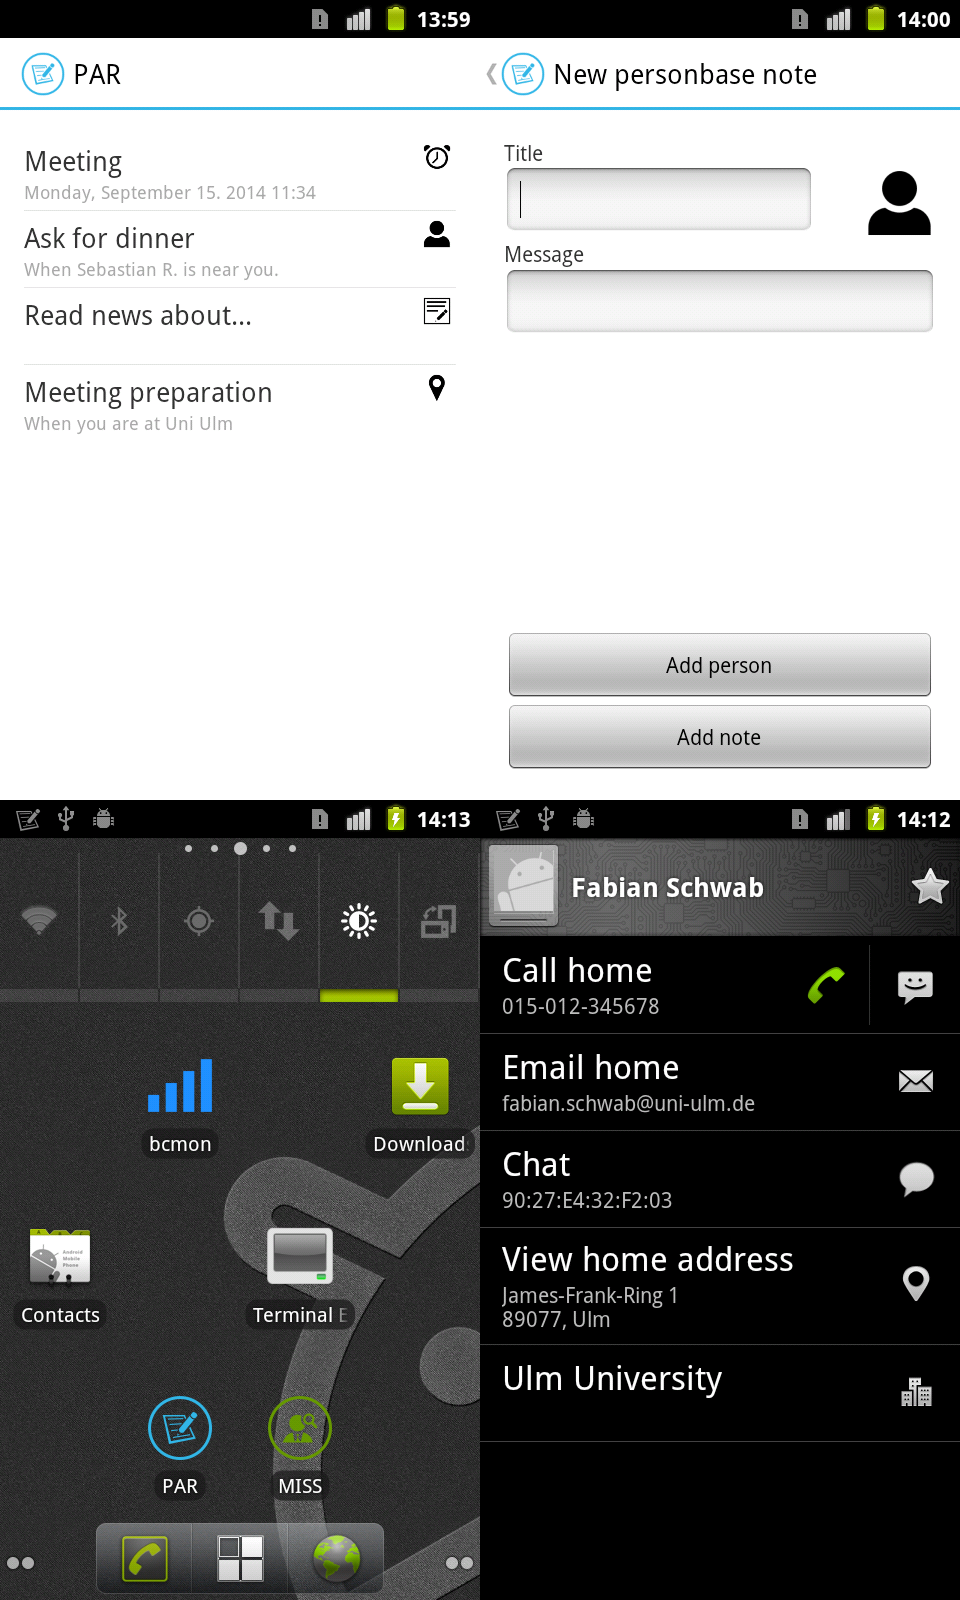
\includegraphics[width=3.0in]{bilder/par.png}
    \caption{Screenshots der Anwendung PAR und Notifikation in der Statusleiste.}
    \label{fig:par}
\end{figure}
\chapter{Zusammenfassung und Ausblick}
In diesem Projekt wurde ein Service für das mobile Betriebssystem Android entwickelt. Dieser Service benutzt WLAN-Kommunikation um Geräte in seiner Nähe zu erfassen und zu identifizieren. Das wird dadurch ermöglicht, indem die komplette Netzwerkkommunikation in der Umgebung mitgehürt wird. Anhand von bestimmten Paketen können MAC-Adressen anderer Geräte ermittelt und mit MAC-Adressen bekannter Geräte verglichen werden. \\ 
Der Service steht als Hintergrunddienst bereit und kann von beliebigen Anwendungen genutzt werden. Wichtig hierbei ist, dass die Anwendungen korrekt mit dem Service kommunizieren. Die Kommunikation findet über ein Anfrage-Antwort Schema statt. \\
Mit dem im Zuges des Projekts entwickelten Services und einer Beispielanwendung, die diesen Service verwendet, konnte das zu Beginn beschriebene Problem gelöst werden. Es lassen sich MAC-Adressen von WLAN-fähigen Geräten übergeben, die anschließend vom Service gesucht werden. Befindet sich ein Gerät in der Nähe, wird die Anwendung vom Service benachrichtigt und der Nutzer wird wiederum von der Anwendung über den Fund informiert. \\\\
Ein großen Problem das aktuell besteht, ist die Geräteabhängigkeit und die damit einhergehende Limitierung auf Android 2.3.3. Würde Google für zukünftige Versionen des Betriebssystems eine Schnittstelle anbieten um den \textit{Monitor Mode} zu aktivieren, wäre dieses kein Problem mehr, da hierdurch die Implementierung des \textit{Monitor Modes} im Gerätetreiber zwingend wäre.
\section{Ausblick}
Der Service ist in seinen Grundzügen gut nutzbar, hat aber dennoch er ein paar offensichtliche Schwachstellen. Diese Schwachstellen könnten aber durch eine Weiterentwicklung gelöst werden. So können zum Beispiel beim Abtippen der MAC-Adresse Fehler gemacht werden. Ein falscher Buchstabe oder eine falsche Zahl kann dazu führen, dass das eigentliche Gerät nicht mehr gefunden werden kann. \\
Um dies auszuschließen, könnte das Einlesen der MAC-Adresse automatisiert werden. Durch ein vorherigen Suchvorgang könnten alle in der Nähe befindlichen Geräte aufgelistet und das Richtige anschließend ausgewählt werden. Eine weitere Möglichkeit das Problem anzugehen wäre eine alternative Verbindung, wie beispielsweise NFC oder Bluetooth, um die MAC-Adresse zwischen den betreffenden Geräten auszutauschen.\\
Ebenso kann durch einen aktivierten \textit{Moditor Mode} kein Datenaustausch mehr über das WLAN Netz erfolgen. Dieser wird dann vom Betriebssystem automatisch auf das Mobilfunknetz ausgelagert. Um eine WLAN Nutzung weiterhin zu ermöglichen, wäre es sinnvoll bekannte Netzwerke zu suchen und den \textit{Monitor Mode} dann, je nach Bedarf, zu deaktivieren. Beispielsweise könnte bei aktivem Display der \textit{Monitor Mode} deaktiviert werden. 
Ebenfalls könnte der Service noch um eine Funktion erweitert werden, mit dem sich der \textit{Monitor Mode} automatisch in begrenzten Zeitintervallen an- und abschalten lässt. Dies schont die Batterie und trägt zu einer längeren Laufzeit des Gerätes bei. \\ 
\bibliographystyle{plain}
\bibliography{document}
\end{document}
